\documentclass[conference]{IEEEtran}
\IEEEoverridecommandlockouts
% The preceding line is only needed to identify funding in the first footnote. If that is unneeded, please comment it out.
\usepackage{cite}
\usepackage{amsmath,amssymb,amsfonts}
\usepackage{graphicx}
\usepackage{textcomp}
\usepackage{enumitem}
\usepackage{xcolor}
\usepackage{times}
\usepackage{siunitx}
\usepackage{latexsym}
\usepackage{hyperref}
\usepackage{algpseudocode}
\usepackage{algorithm}
\usepackage{caption}
\usepackage{subcaption}
\algnewcommand\algorithmicforeach{\textbf{for each}}
\algdef{S}[FOR]{ForEach}[1]{\algorithmicforeach\ #1\ \algorithmicdo}
\def\BibTeX{{\rm B\kern-.05em{\sc i\kern-.025em b}\kern-.08em
    T\kern-.1667em\lower.7ex\hbox{E}\kern-.125emX}}

\begin{document}

\title{Comparative study of Dask and Spark for neuroimaging pipelines\\
{\footnotesize \textsuperscript{*}Note: Sub-titles are not captured in Xplore and
should not be used}
\thanks{Natural Sciences and Engineering Research Council}
}

\author{\IEEEauthorblockN{1\textsuperscript{st} Mathieu Dugr\'e}
\IEEEauthorblockA{\textit{Computer Science and Software Engineering} \\
\textit{Concordia University}\\
Montreal, Canada \\
mathieu.dugre@mail.concordia.ca}
\and
\IEEEauthorblockN{2\textsuperscript{nd} Given Name Surname}
\IEEEauthorblockA{\textit{Computer Science and Software Engineering} \\
\textit{Concordia University}\\
Montreal, Canada \\
email address}
\and
\IEEEauthorblockN{3\textsuperscript{rd} Given Name Surname}
\IEEEauthorblockA{\textit{Computer Science and Software Engineering} \\
\textit{Concordia University}\\
Montreal, Canada \\
email address}
}

\maketitle

\begin{abstract}
% Topic
As the amount of data increases and is easier to access, Big Data processing becomes
critical in neuroimaging.
% Problem
This is an issue as the currently used frameworks are specialized for neuroimaging
and not Big Data concerns. This can lead to performance decrease or limit the
research we can perform.
% Relevance
The usage of Big Data framework is beneficial to this problem. The state-of-the-art
general purpose Big Data framework Spark has its code base written in Scala, while
our laboratory mostly uses Python. This can be problematic since it is harder to port
our pipelines to the framework. Also, theoretically, it leads to performance decrease.

% Approach
We propose to use Dask since it provides native Python parallelism to pipelines while
providing support to familiar API from Python's scientific ecosystem. Unfortunately,
there are few comparisons between Spark and Dask; especially in neuroimaging.
Moreover, these studies were done when Dask was still an immature framework which
makes those studies unfair nowadays. This is our motivation to compare the latest
version of Dask with Spark.
% Methods (one sentence)
To evaluate the frameworks, we focus on their performance and their scheduler.

% Key Impact
Our study demonstrates the potential of using Dask as the framework to build
neuroimaging pipelines.
\end{abstract}

\begin{IEEEkeywords}
Big Data, Dask, Spark, performance, neuroimaging
\end{IEEEkeywords}

\section{Introduction}
% Context
With the increasing number of data available in neuroimaging,~\cite{ALFAROALMAGRO:18,
UKBioBank:18} the processing of Big Data becomes critical. Frameworks like
Nipype~\cite{Nipype:11} are usually used to create neuroimaging pipelines however it
is worth considering the use of general purpose Big Data
frameworks~\cite{Hayot-Sasson:17}. In that research, Spark~\cite{Spark:16} was a
natural choice as it is the state-of-the-art framework for Big Data. Since our
laboratory mostly works with Python, we want to know if Dask~\cite{Dask:15}, a Python
written framework, could bring better or similar performances while facilitating
usage.

%Similarities
Spark and Dask offer in-memory computing, data locality, and lazy evaluation; which
is common for Big Data framework. Both their scheduler operates dynamically. This is
good when the runtimes are not known ahead of time~\cite{Dask:15}. Over these
similarities, the frameworks are quite different.

% Spark
On the one hand, we have Spark which provides a high-level API. This allows the
scheduler to perform more optimizations which makes it well suited for neuroimaging
analysis that often requires the usage of a pipeline with multiple steps. Though,
Spark's code base is in Scala which theoretically can lead to slow down in execution
due to a required serialization. Moreover, while Spark's API is flexible and allows
most implementations, it differs from the ones seen in Python's ecosystem.

% Dask
On the other hand, Dask was created with the purpose of natively parallelize Python
pipelines while keeping the syntax of familiar API from Python's scientific
ecosystem. However, Dask is still a young framework with work to be done; it's API
does not completely replicate the library it supports. While its lower-level API
allows the implementation of more complex algorithms it sacrifices a layer of
optimization.
% Related work
Previous work shows that Dask had significant overhead and was
hard to debug~\cite{Mehta:17}.
% What issues your work addresses
Dask was immature at the time and a lot of change was brought to the framework.
Therefore we think it is valuable to re-compare it with Spark.

%% Dask API
The Dask APIs we decide to use for our comparison are Dask bag, delayed and futures.
Dask bag offers an easy API to parallelize data. Dask delayed offer a lower-level API
that offers more flexibility; this is good to implement more complex tasks that do
not fit in the Dask bag framework. Dask futures is a real-time API. Both Dask bag and
delayed apply lazy evaluation to tasks while futures trigger them directly.

% Methods used (summary)
The project aims to compare the state-of-the-art general-purpose framework Spark with
the newcomer Dask. We decide to compare the performance of Spark and Dask on a custom
incrementation pipeline to simplify the effect of the algorithm on the comparison.
Then we assess the frameworks on two real-life applications: (1) histogram of the
voxels intensity in a 3d images (2) BIDS example.

% Implications of our research
The result from our project help in deciding if Dask is a good choice to build
neuroimaging pipelines.


%%%%% MATERIAL AND METHODS %%%%%%
\section{Material and Methods}

\subsection{Engines}
For all our experiments, we used Spark v2.4.0 and Dask v1.1.4.

\subsubsection{PySpark RDD~\cite{spark-rdd}} Spark is a general-purpose Big Data
framework. It provides in-memory computing, data locality and lazy evaluation. Spark
abstracts resilient distributed dataset (RDD)~\cite{RDD} making it fault-tolerant. Its
high-level API provides optimizations for transformations applied data. Since
Spark is written in Scala, this optimization is lessen because it requires a
serialization from Python to Java. The API offered by Spark is flexible and suits most
problems however it differs from Python ecosystem. The standalone scheduler is used for
our experiment. It has a LIFO policy.

\subsubsection{Dask Bag~\cite{dask-bag}} Dask Bag is one of the high-level API
offered by Dask. Like Spark, it provides in-memory computing, data locality and lazy
evaluation however it does not have fault resilience. Fundamently, it is parallized
lists. Dask Bag parallelizes computations of large collection of generic python
objects~\cite{dask-bag}. Also, it offers optimized algorithms that mimic most of the
toolz~\cite{toolz} library. Our experiment use the Dask Distributed~\cite{dask-distributed}
scheduler. It has a LIFO policy. In theory it should speed-up the pipeline excution
by finishing a branch of task computations before starting new ones.

\subsubsection{Dask Delayed~\cite{dask-delayed}} Dask Delayed is a low-level API. It
does not offer the optimized algorithm as the high-level APIs however it allows the
user to parallelize custom function that do not fit in the array, dataframe or
MapReduce framework. This is perfect for more complex function which could easily be
parallelized. Like Dask Bag, it offers in-memory computing, data locality and lack
fault resilience. The Dask Distributed scheduler is used.

\subsubsection{Dask Futures~\cite{dask-futures}} Dask Futures is also a low-level API
from Dask. Like the other Dask APIs, it benifits of in-memory computing and data
locatlity. However, unlike the other APIs, Dask Futures triggers computation
immediately. When the user tries to gather data if available it will return the
result otherwise it will block until the computation is done. Again, the Dask
Distributed scheduler is used.


\subsection{Dataset}
For the incrementation and histogram experiment the BigBrain~\cite{Amunts:13} is
used. It is a three-dimensional image of a brain scanned at \SI{40}{\micro\metre}.
The data set store the intensity of each voxel and their position. This results in a
75GB image. It is stored in 125 chunks in the \textit{MINC}~\cite{minc} format. To
perform our experiment we convert the chunks into the \textit{NifTI}~\cite{nifti}
format. Also, using \textit{sam}~\cite{sam} we combine the chunks and split them into
30, 125 and 750 chunks of equal size; each of 2.5GB, 0.6GB, and 0.1GB, respectively.

\subsection{Applications}
%% Incrementation
\subsubsection{\textbf{Incrementation}}
As our first experiment to benchmark the frameworks, we used a simple incrementation
pipeline (see Algorithm~\ref{alg:incrementation}). It reads chunks from the BigBrain
image, increments the intensity value of each voxel by 1 for a specified amount of
iterations, and write the result to an NFS as a NifTI image. Incrementing the data
reduce the caching effect. This experiment allows us to study the behavior of the
frameworks when all input are processed independently; i.e.\ each task in the graph
only depends on the previous one (see Figure~\ref{fig:tg-inc}). This mimic the
behavior of analyzing multiple independent subjects in parallel.

This experiment refers to the implementation of the Spark pipelines purposed
in Ref.~\cite{Hayot-Sasson:17}.

\begin{algorithm}[!b]
    \caption{Incrementation}\label{alg:incrementation}
    \begin{algorithmic}
    \Require{\(x\), a sleep delay in float}
    \Require{\(file\), a file containing a chunk}
    \Require{\(fs\), NFS to write image to.}
    \State{Read \(chunk\) from \(file\)}
    \ForEach{\(i \in iterations\)}
        \ForEach{\(chunk \in image\)}
            \State{\(chunk\gets chunk+1\)}
            \State{Sleep \(x\)}
        \EndFor
    \EndFor
    \State{Write \(chunk\) to \(fs\)}
\end{algorithmic}
\end{algorithm}

\begin{figure}[!b]
    \centering
    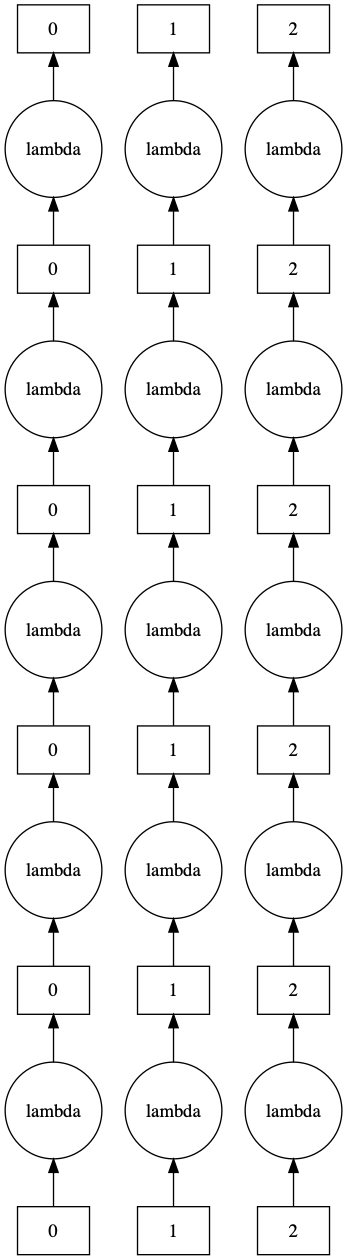
\includegraphics[width=0.125\textwidth,
    angle=-90]{images/incrementation-task-graph.png}
    \caption{Task graph for Incrementation}\label{fig:tg-inc}
\end{figure}

\subsubsection{\textbf{Histogram}}
Our second experiment consist to calculate the histogram of the intensity of the
voxel in BigBrain (see Algorithm~\ref{alg:histogram}). It reads the images from the
nfs, calculate inividual image frequency, aggregate the images frequency together,
and write the result to a file. In this experiment, the result depends on all the
input (see Fig.~\ref{fig:tg-histo}). This allows to study the behavior of the
frameworks when tasks are dependent. Also, this application requires data shuffling
thus inter-worker communication. We decided to omit Dask Futures as it does not had
any value over Dask Delayed in this application.

\begin{algorithm}[!t]
    \caption{Histogram}\label{alg:histogram}
    \begin{algorithmic}
    \Require{\(files\), files containing BigBrain}
    \Require{\(fs\), NFS to save image to.}
    \ForEach{\(file \in files\)}
        \State{Read \(chunk\) from \(file\)}
        \State{{Calculate \(frequency\) of \(chunks\)}}
    \EndFor
    
    \State{\(histogram\gets\)Aggregate \(frequency\) of each \(file\)}

    \State{Write \(histogram\) to \(fs\)}
    \end{algorithmic}
\end{algorithm}

\begin{figure}[!t]
    \centering
    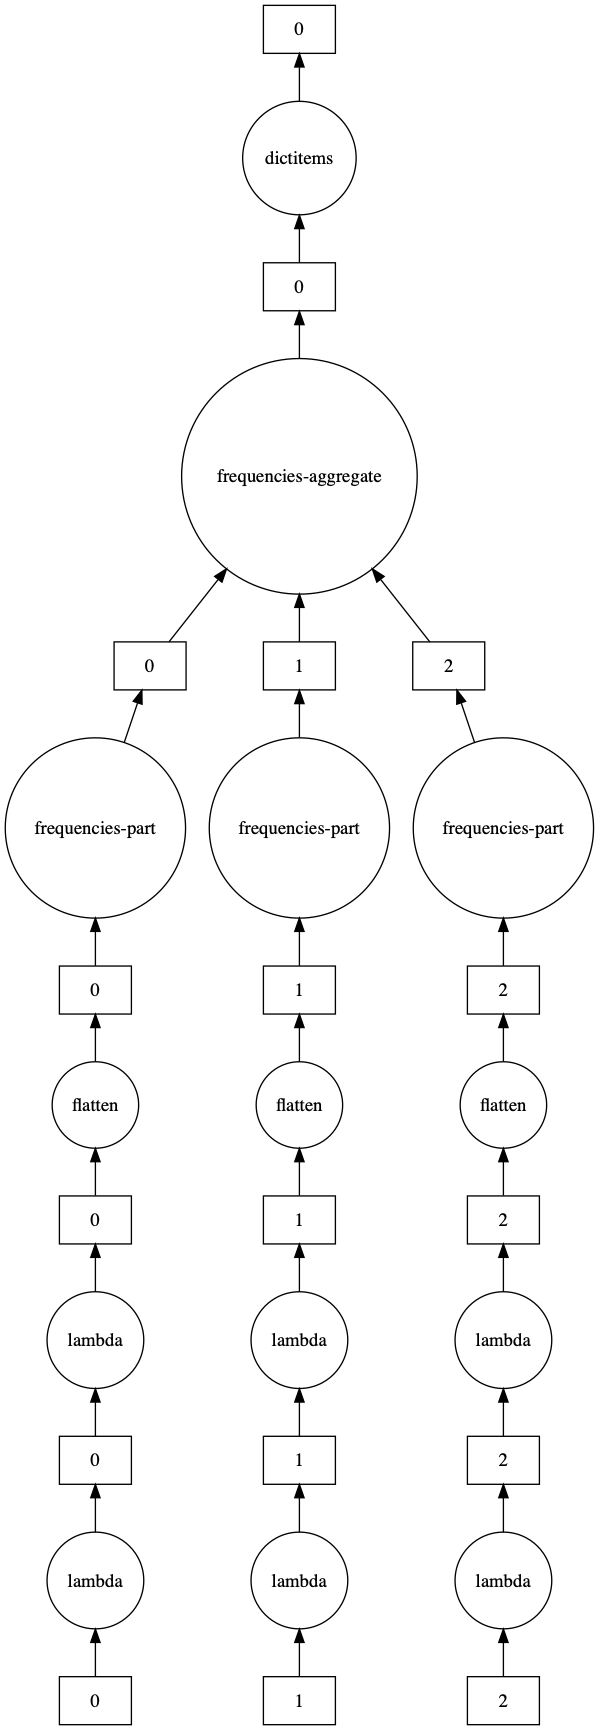
\includegraphics[width=0.16\textwidth, angle=-90]{images/histogram-task-graph.png}
    \caption{Task graph for Histogram}\label{fig:tg-histo}
\end{figure}

\subsection{Experiment}
The applications are benchmarked according to up to four parameters
(Table~\ref{tab:param}):

\textbf{Number of workers:} Varying the numbers of workers helps in assessing the
scaling of the frameworks in a cluster. Also, it helps in determining the level of
parallelism of the frameworks.

\textbf{Number of chunks:} Evaluating the frameworks on different amount of chunks
allows us to understand their behavior with different task size and IO requirements.

\textbf{Number of iterations:} We change the amount of iterations for the
incrementation~\ref{alg:incrementation} to study the effect of the job size.

\textbf{Sleep delay:} We modify the sleep delay in the
incrementation~\ref{alg:incrementation} to understand the behavior of task of
different length.

The baseline for our experiments is: 8 workers, 125 chunks, 10 iterations and 4
seconds sleep delay.


\begin{table}[!b]
    \renewcommand{\arraystretch}{1.3}
    \caption{Parameters for the experiments}\label{tab:param}
    \centering
    \begin{tabular*}{\columnwidth}{llll}
    \hline
                        & Incrementation & Histogram             & BIDS Example          \\ \hline
    \# of worker        & 1, 2, 4, 8     & 1, 2, 4, 8            & 1, 2, 4, 8            \\
    \# of chunks        & 30, 125, 750   & 30, 125, 750          & 30, 125, 750          \\
    \# of iterations    & 1, 10, 100     & \multicolumn{1}{c}{-} & \multicolumn{1}{c}{-} \\
    Sleep delay {[}s{]} & 1, 4, 16, 64   & \multicolumn{1}{c}{-} & \multicolumn{1}{c}{-} \\ \hline
    \end{tabular*}
    \end{table}


\subsection{Infrastructure}
All experiments were performed on Arbutus Cloud Compute Canda. Each node has CentOS
7.5.1804 as base operating system and have the Linux kernel version
3.10.0\-862.11.6.el7.x86\_64. The nodes have an Intel Xeon Gold 6130 processor with
30GB 2666 MHz memory. The networks has a 10GB/s bandwidth. The filesystem is 2TB NFS v4.



%%%%% RESULTS %%%%%
\section{Results}

%%% INCREMENTATION %%%
%% worker
\subsection{Experiment 1: Number of instances}
Figure~\ref{fig:inc_worker}(a) shows that the increase in performance is not
proportional to the number of workers which differ from what we would expect; it even
decrease when we reach 8 workers. This is explained by an increase in IO overhead
correlated to the number of workers (Figure~\ref{fig:inc_worker}(b)), as more worker
access the NFS simultaneously it increases the stress put on the system which results
in bottleneck, errors and slow down.

On the one hand, Dask seems better when using a single worker. On the other hand,
Spark makespan decreases faster for a higher level of parallelism. Dask is constantly
faster than Spark which makes us think it has a better scheduler.

\begin{figure}[!t]
    \centering
    \begin{subfigure}[b]{\columnwidth}
        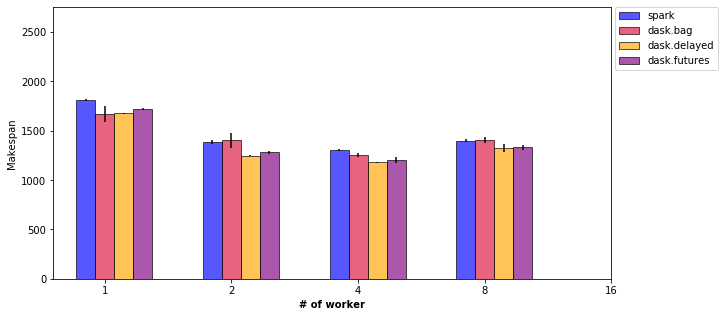
\includegraphics[clip,width=\columnwidth]{images/inc_worker.png}%
        \caption{Incrementation makespan}\label{fig:inc_ms_worker}
    \end{subfigure}
    \\
    \begin{subfigure}[b]{\columnwidth}
        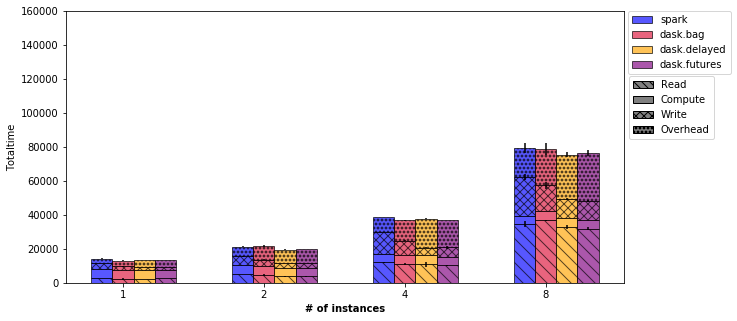
\includegraphics[clip,width=\columnwidth]{images/inc_idle_worker.png}%
        \caption{Incrementation total time}\label{fig:inc_tt_worker}
    \end{subfigure}
    \caption{125 chunks, 10 iterations, 4 sec.\ sleep delay}\label{fig:inc_worker}
\end{figure}

% Chunks
\subsection{Experiment 1: Number of chunks}
In Figure~\ref{fig:inc_chunk} Spark is not compared for 30 chunks. This is because
Spark has a 2GB limitation in the task size it can compute. Note from
Figure~\ref{fig:inc_chunk}(b) that the compute time increase when there are more
chunks. This is expected because the sleep delay is constant throughout this
experiment and there are more compute tasks when the number of chunks increases. We
also note that in Figure~\ref{fig:inc_tt_chunk} for 30 chunks the Dask bag API has a
much lower overhead time. This is because we only calculate the idle time of the used
core. Dask bag was only using one thread per block in comparison to Dask delayed and
Dask futures which was offloading the calculations on multiple threads of the same
worker. From Figure~\ref{fig:inc_chunk} we observe that when the dataset is separated
in more (smaller) chunks it saves IO time however it increases the overhead by a
similar amount; the inverse happens when we reduce the number of chunks.

\begin{figure}[!t]
    \centering
    \begin{subfigure}[b]{\columnwidth}
        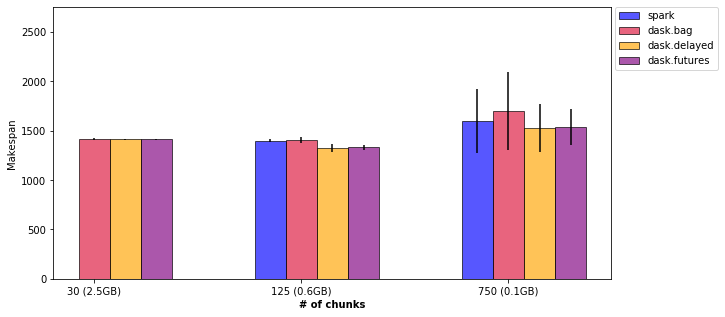
\includegraphics[clip,width=\columnwidth]{images/inc_chunk.png}%
        \caption{Incrementation makespan}\label{fig:inc_ms_chunk}
    \end{subfigure}
    \\
    \begin{subfigure}[b]{\columnwidth}
        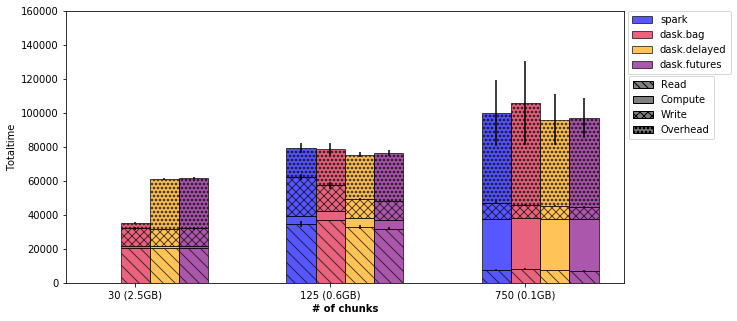
\includegraphics[clip,width=\columnwidth]{images/inc_idle_chunk.png}%
        \caption{Incrementation total time}\label{fig:inc_tt_chunk}
    \end{subfigure}
    \caption{10 iterations, 4 sec.\ sleep delay, 8 instances}\label{fig:inc_chunk}
\end{figure}

%% Iterations
\subsection{Experiment 1: Number of iterations}
In Figure~\ref{fig:inc_itr}, Spark and the Dask bag API are equivalent in terms of
performance. The Dask delayed API seems to perform well with a low amount of task but
grow faster the Spark and Dask bag. We think this is because Dask delayed often
schedule a block on a different thread of the same worker which causes small delays
every time due to inter-thread data communication. This is good when there are fewer
tasks as is make the IO between blocks go out of sync hence lowering the IO
bottleneck however as the number of tasks increases those small delays become
significant. The Dask futures API seems to outperform all the other APIs but this is
most likely because the tasks are not interdependent thus this application benefits
from the less optimal but faster scheduling brought by Dask futures.

\begin{figure}[!t]
    \centering
    \begin{subfigure}[b]{\columnwidth}
        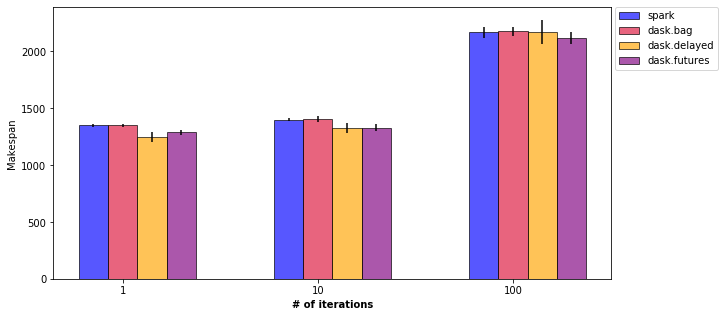
\includegraphics[clip,width=\columnwidth]{images/inc_itr.png}%
        \caption{Incrementation makespan}\label{fig:inc_ms_chunk}
    \end{subfigure}
    \\
    \begin{subfigure}[b]{\columnwidth}
        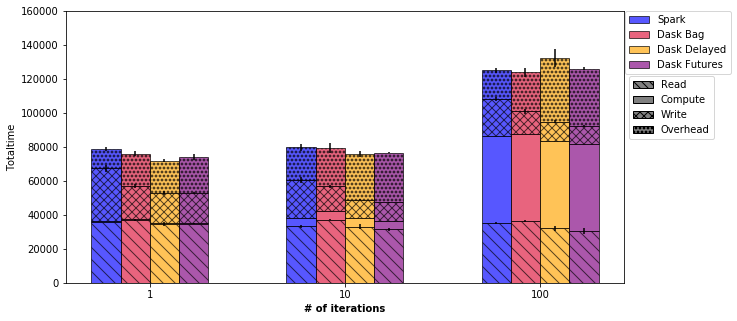
\includegraphics[clip,width=\columnwidth]{images/inc_idle_itr.png}%
        \caption{Incrementation total time}\label{fig:inc_tt_chunk}
    \end{subfigure}
    \caption{125 chunks, 4 sec.\ sleep delay, 8 instances}\label{fig:inc_itr}
\end{figure}


%% Sleep time
\subsection{Experiment 1: Sleep delay}
As Figure~\ref{fig:inc_sleep}(b) and Table~\ref{tb:inc-sleep} shows Spark has the
smallest overhead all around and it is also the one that reduces the most with longer
task length. In term of overhead, Dask bag trailing slightly behind Spark although is
better than Dask delayed and Dask futures. The opposite happens for the IO time.
% Not sure what to conclude.

%%%% CHANGE NUMBER
\begin{table}[!t]
    \renewcommand{\arraystretch}{1.3}
    \caption{Distribution of the execution time in seconds for our baseline: 125
    chunks, 4 sec.\ sleep delay, 10 iterations, and 8 workers}\label{tb:inc-sleep}
    \centering
    \begin{tabular*}{\columnwidth}{llllll}
    \hline
                 & Read  & Compute & Write & Overhead & Total \\ \hline
    Spark        & 34465 & 5118    & 22679 & 17076    & 79338 \\
    Dask.bag     & 36863 & 5121    & 15449 & 21388    & 78821 \\
    Dask.delayed & 32769 & 5119    & 11373 & 26199    & 75461 \\
    Dask.futures & 31891 & 5120    & 11270 & 27984    & 76265 \\ \hline
    \end{tabular*}
 \end{table}

\begin{figure}[!t]
    \centering
    \begin{subfigure}[b]{\columnwidth}
        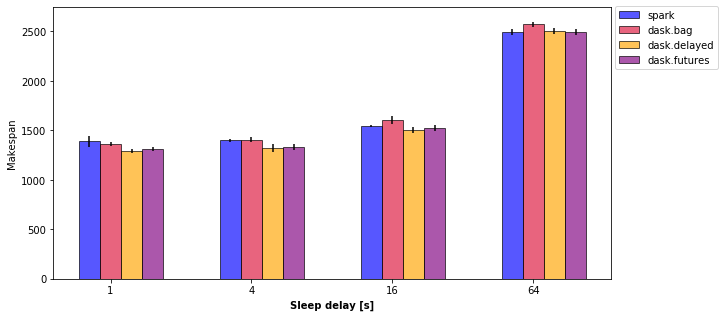
\includegraphics[clip,width=\columnwidth]{images/inc_sleep.png}%
        \caption{Incrementation makespan}\label{fig:inc_ms_chunk}
    \end{subfigure}
    \\
    \begin{subfigure}[b]{\columnwidth}
        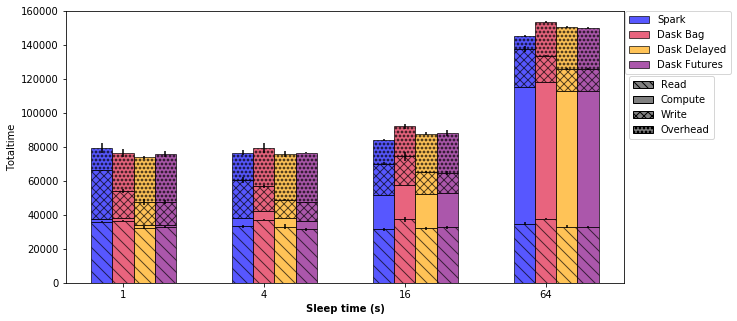
\includegraphics[clip,width=\columnwidth]{images/inc_idle_sleep.png}%
        \caption{Incrementation total time}\label{fig:inc_tt_chunk}
    \end{subfigure}
    \caption{125 chunks, 10 iterations, 8 instances}\label{fig:inc_sleep}
\end{figure}

%% Baseline gantt chart
\subsection{Experimentation 1: Baseline timeline}
From Table~\ref{tb:inc_base} and Figure~\ref{fig:inc_gantt}, the frameworks have
similar makespan however the time spend for each type of task differs significantly.
Spark tends to spend more time than other frameworks for IO however it has a much
lower overhead. Dask delayed and futures have the lowest IO time but a much higher
overhead. Dask bag stands in the middle for both IO and overhead. Compute time is
approximately the same for all frameworks.

\begin{table}[!t]
    \renewcommand{\arraystretch}{1.3}
    \caption{Distribution of the execution time in seconds for our baseline: 125
    chunks, 4 sec.\ sleep delay, 10 iterations, and 8 workers}\label{tb:inc_base}
    \centering
    \begin{tabular*}{\columnwidth}{llllll}
    \hline
                    & Read  & Compute & Write & Overhead & Total \\ \hline
    Spark        & 34465 & 5118    & 22679 & 17076    & 79338 \\
    Dask.bag     & 36863 & 5121    & 15449 & 21388    & 78821 \\
    Dask.delayed & 32769 & 5119    & 11373 & 26199    & 75461 \\
    Dask.futures & 31891 & 5120    & 11270 & 27984    & 76265 \\ \hline
    \end{tabular*}
 \end{table}

\begin{figure*}[!t]
    \centering
    \begin{subfigure}[b]{\columnwidth}
        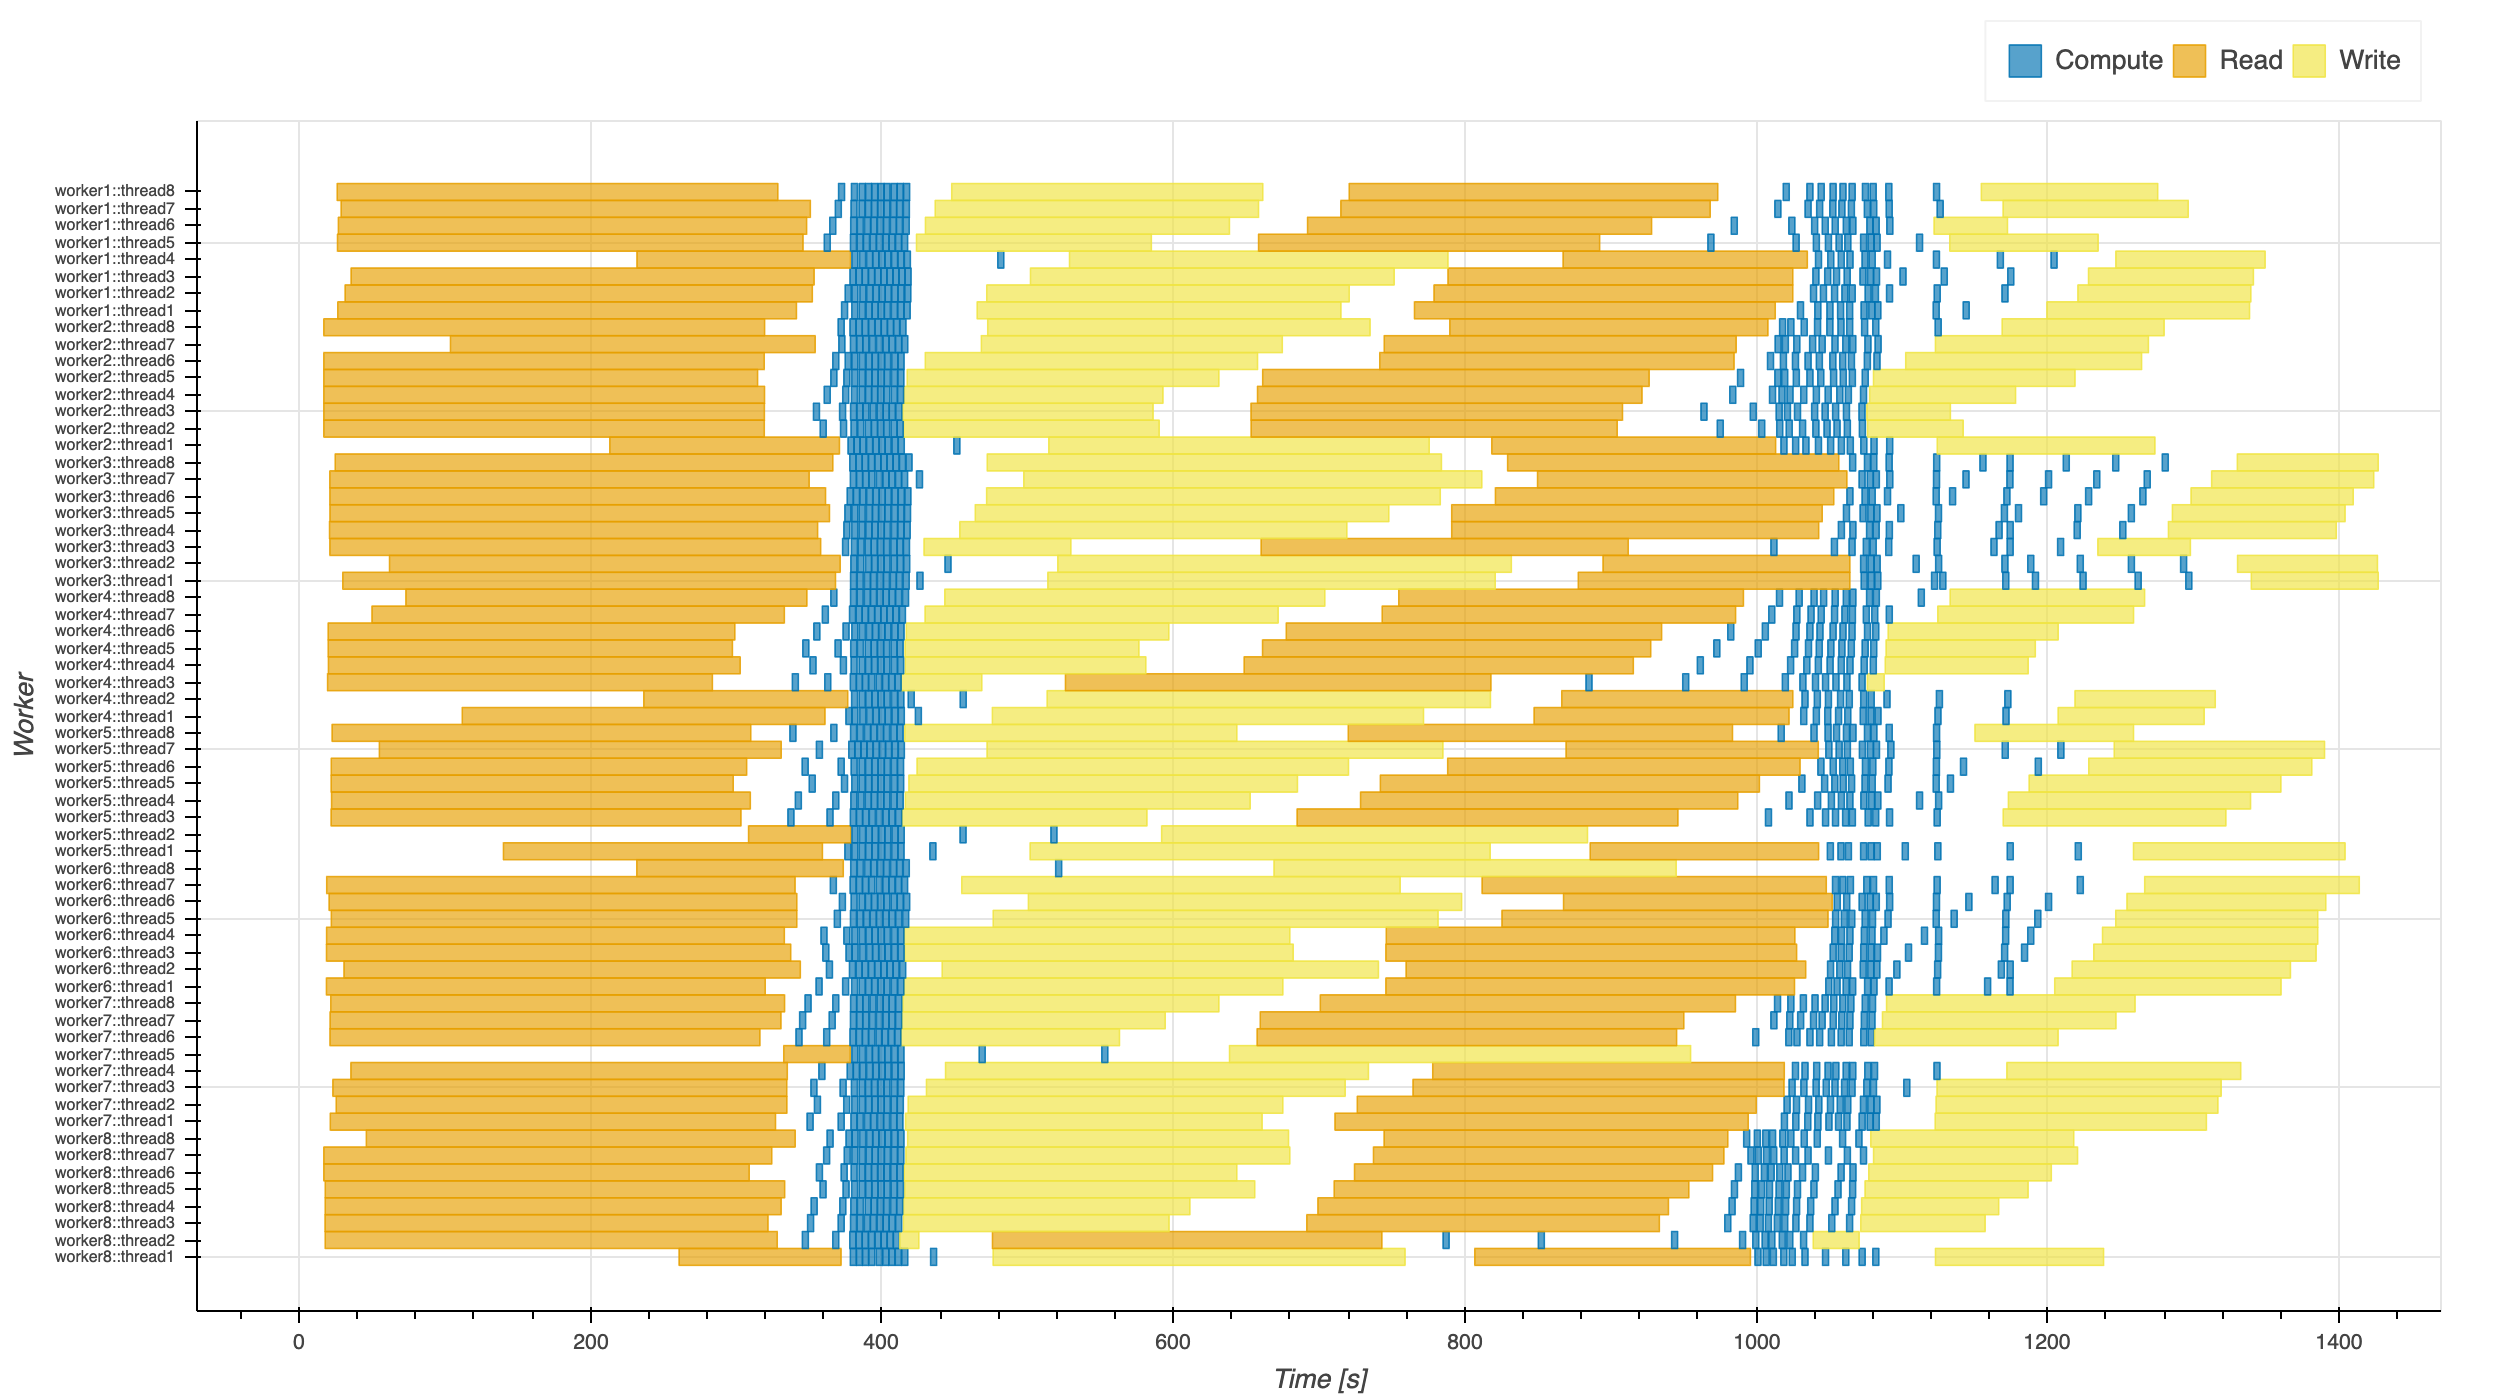
\includegraphics[clip,width=\columnwidth]{images/spark_inc_baseline_gantt.png}
        \caption{Spark execution timeline}\label{fig:inc_spark_gantt}
    \end{subfigure}
    \hfill
    \begin{subfigure}[b]{\columnwidth}
        \includegraphics[clip,width=\columnwidth]{images/Dask_bag_inc_baseline_gantt.png}%
        \caption{Dask bag execution timeline}\label{fig:inc_dask_bag_gantt}
    \end{subfigure}
    \\
    \begin{subfigure}[b]{\columnwidth}
        \includegraphics[clip,width=\columnwidth]{images/Dask_delayed_inc_baseline_gantt.png}%
        \caption{Dask delayed execution timeline}\label{fig:inc_dask_delayed_gantt}
    \end{subfigure}
    \hfill
    \begin{subfigure}[b]{\columnwidth}
        \includegraphics[clip,width=\columnwidth]{images/Dask_futures_inc_baseline_gantt.png}%
        \caption{Dask futures execution timeline}\label{fig:inc_dask_futures_gantt}
    \end{subfigure}
    \caption{125 chunks, 4 sec.\ sleep delay, 8 instances}
\end{figure*}


%%% HISTOGRAM %%%
\subsection{Experiment 2: Number of instances}

\begin{figure}[!t]
    \centering
    \begin{subfigure}[b]{\columnwidth}
        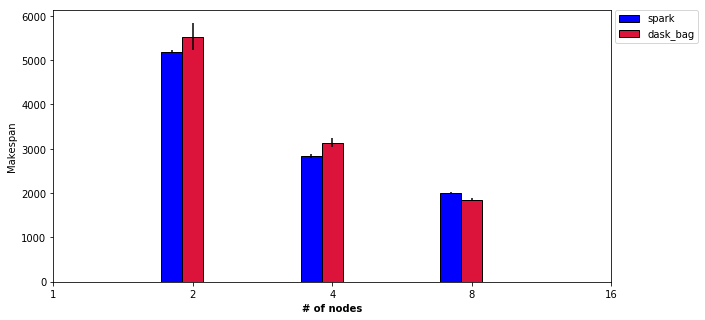
\includegraphics[clip,width=\columnwidth]{images/histo_instance.png}%
        \caption{Histogram makespan}\label{fig:histo_ms_worker}
    \end{subfigure}
    \\
    \begin{subfigure}[b]{\columnwidth}
        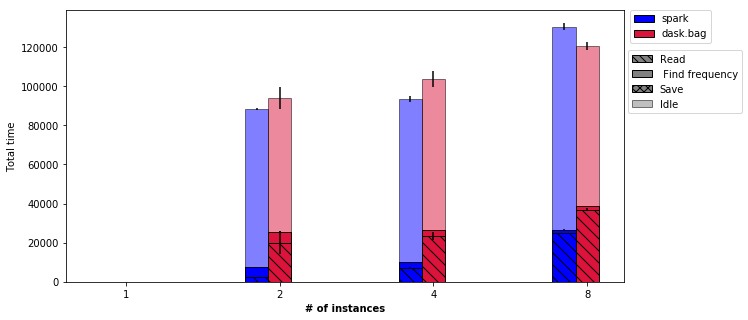
\includegraphics[clip,width=\columnwidth]{images/histo_idle_instances.png}%
        \caption{Histogram total time}\label{fig:histo_tt_worker}
    \end{subfigure}
    \caption{125 chunks}
\end{figure}

\subsection{Experiment 2: Number of chunks}

\begin{figure}[!t]
    \centering
    \begin{subfigure}[b]{\columnwidth}
        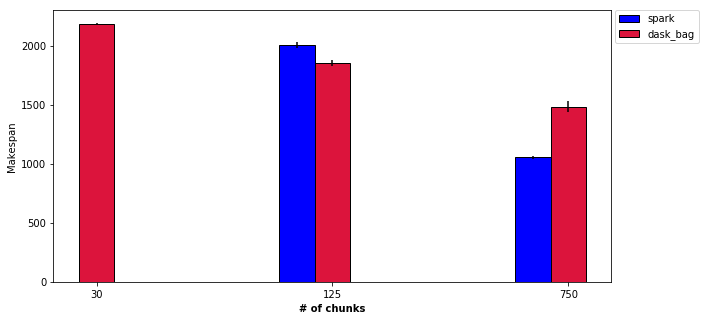
\includegraphics[clip,width=\columnwidth]{images/histo_splits.png}%
        \caption{Histogram makespan}\label{fig:histo_ms_chunk}
    \end{subfigure}
    \\
    \begin{subfigure}[b]{\columnwidth}
        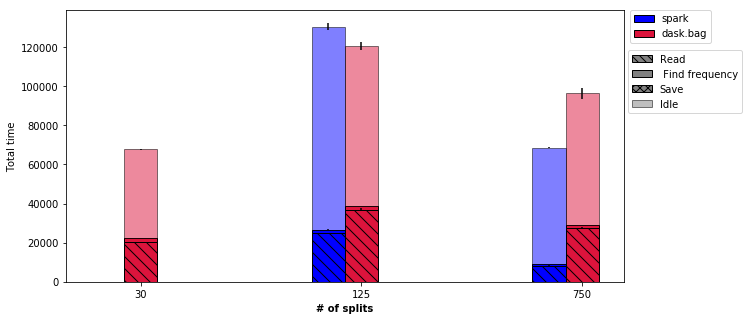
\includegraphics[clip,width=\columnwidth]{images/histo_idle_splits.png}%
        \caption{Histogram total time}\label{fig:histo_tt_chunk}
    \end{subfigure}
    \caption{8 workers}
\end{figure}

%%% BIDS EXAMPLE %%%
\subsection{Experiment 3: Number of instances}



%%%%% DISCUSSION %%%%%
\section{Discussion}
\subsection{IO Time}


\subsection{Serialization}
We think that serialization could have an important effect on the makespan of the
application. This could potentially slow down the application when a lot of tasks are
scheduled.

\subsection{NFS}
The NFS seems to be a source of the bottleneck. We think that exploring another file
system, like Lustre, could give us insight into the actual effect of the NFS on the
application makespan. We also think that the NFS caching could play an effect on the
task of different lengths.

\subsection{Scheduler}
The Dask scheduler seems to have some bizarre behavior. It seems like it waits to
schedule tasks. It could also be due to tasks being scheduled on other workers
thus requiring data to be sent over the network; which would explain the stall on the
worker. More work would be needed to investigate that issue.


\subsection{Caching}
We think that caching plays an effect on the results. As seen in the Gantt chart
previously, some of the read tasks are significantly shorter than others while all
chunks are of equal size.

\section*{Acknowledgment}

We would like to thanks Compute Canada Cloud for the infrastructure.

\section*{References}
\bibliographystyle{IEEEtran}
\bibliography{IEEEabrv,reference}

\end{document}
